\chapter{Cold Electronics}
\label{ch:ce}

%
%%%%%%%%%%%%%%%%%%%%%%%%%%%%%%%%
\section{Introduction}
\label{sec:ce_intro}

\begin{cdrfigure}[The front end electronics as mounted on an APA]{elec_CMBonAPA}{The front end electronics as mounted on an APA.
  {\bf Top:} The front end electronics  is shown in the red circle.
  {\bf Bottom:} Cross section view.}
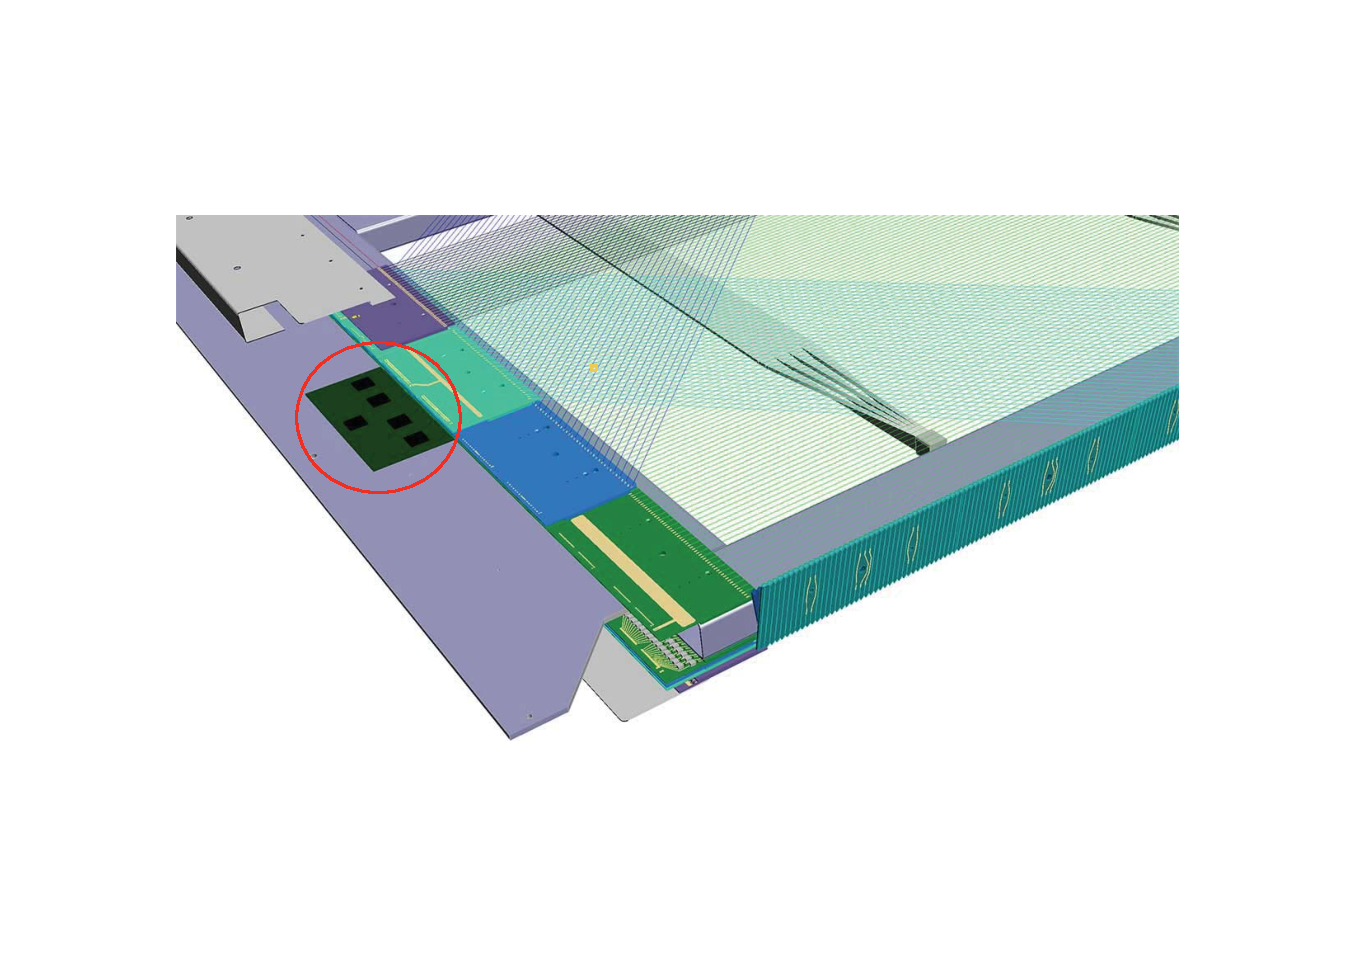
\includegraphics[width=1.00\linewidth]{elec_CMBonAPA_1.pdf}
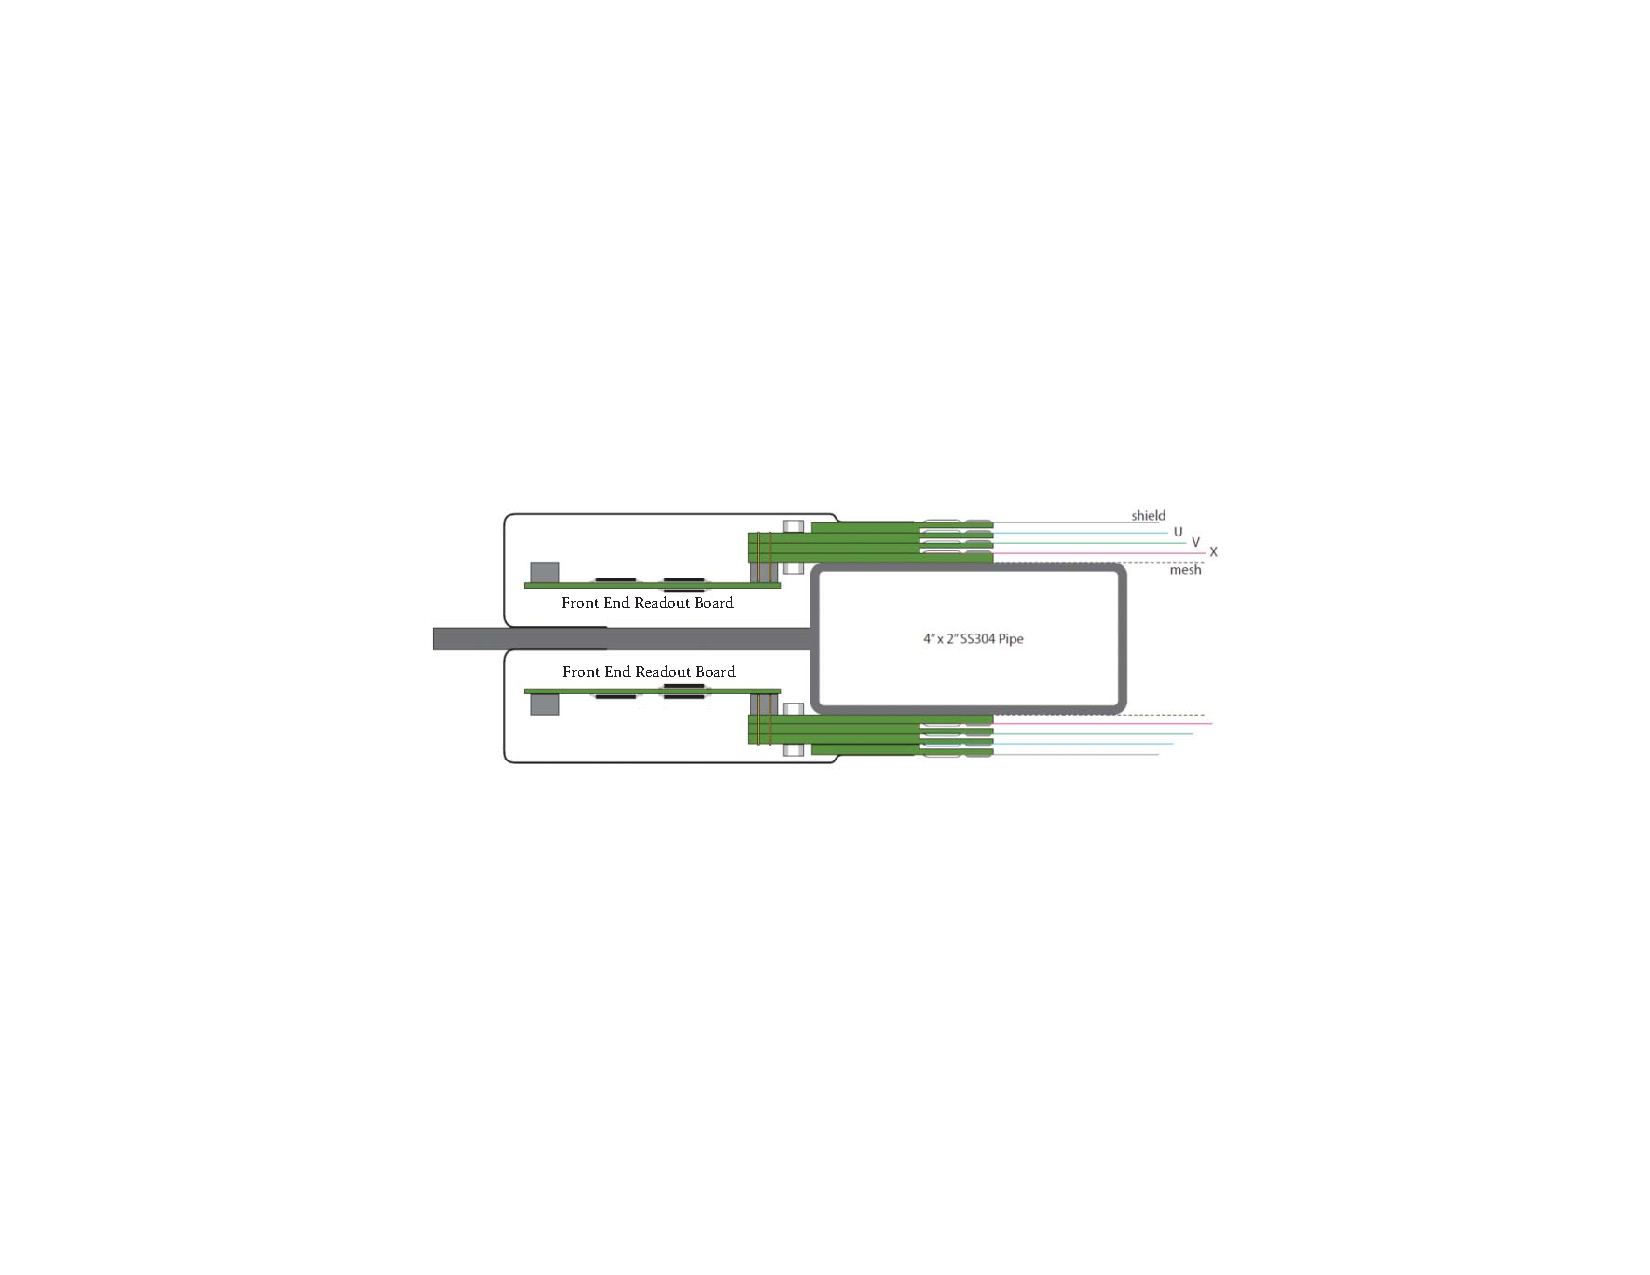
\includegraphics[width=1.00\linewidth]{elec_CMBonAPA_2.pdf}
\end{cdrfigure}

The TPC read-out electronics are referred to as the ``Cold Electronics'' (CE) because they will reside in LAr,
mounted directly on the APA front-end (Figure~\ref{fig:elec_CMBonAPA}).
This will minimize channel capacitance and noise by keeping the length of the connection between an anode wire
and its corresponding electronics input to an absolute minimum.
The CE will be implemented as ASIC chips using CMOS technology,
which performs well at cryogenic temperatures,
and will provide amplification, shaping, digitization, buffering and multiplexing (Mux) of the signals.
Because it is not possible to form a trigger for some important measurements,
such as proton decay and supernova bursts, the CE will be continuously read out,
with a digitized ADC sample from each APA channel (wire) every 500~ns.
For each of the 104 APAs in a 10-kt fiducial cryostat, one cable bundle will connect to the outside of the cryostat through
a feedthrough, with one feedthrough servicing two APAs.
Each of these cable bundles consists of wires for low-voltage power, TPC wire-bias voltages, data-out, clock-in and
digital-control IOs.
% The 2,560 channels from an APA are read out in 20 groups of 128 channels.

The scope of the CE subsystem includes the design, procurement, fabrication, testing,
delivery and installation of the CE, the components of which are:
\begin{itemize}
\item Front-end cards installed on the APAs
\item All electronics on those cards
\item Feedthroughs (a single type, henceforth ``signal feedthroughs'') which handle the signal,
low-voltage power, TPC bias voltage and control lines
\item External interface crates
\item Power supplies, including low-voltage supplies for the CE and bias-voltage supplies for the TPCs
\item Signal, control and power cabling between the front-end cards and the feedthroughs,
and between the feedthroughs and external power supplies and interface crates
\end{itemize}

%
%%%%%%%%%%%%%%%%%%%%%%%%%%%%%%%%
\section{Design Considerations} 
\label{sec:ce_reqs_n_specs}

The requirements for the CE can be found in the requirements documentation \cite{lar-fd-req}.
The most significant ones are listed here. The CE shall:

\begin{itemize}	
\item Provide the means to read out the TPCs and transmit their data in a useful format to the Data Acquisition System (DAQ).
\item Operate for the life of the facility without significant loss of function.
\item Record the channel waveforms continuously without dead time.
\item Use only materials that are compatible with high-purity liquid argon.
\item Provide sufficient precision and range in the digitization to:
\begin{itemize}
\item Discriminate electrons from photon conversions;
\item Optimize for high- and low-energy tracks from accelerator-neutrino interactions;
\item Distinguish a Minimum Ionizing Particle (MIP) from noise with a signal-to-noise ratio $>$ 9:1;
\item Measure the ionization up to 15 times that of a MIP particle, so that stopping kaons from proton decay can be identified.
\end{itemize}
\item Ensure that all power supplies have: 
\begin{itemize}
\item Local monitoring and control
\item Remote monitoring and control through DAQ
\item Over-current and over-voltage protection circuits
\end{itemize}
\item Ensure that the low-voltage (signal) feedthroughs are able to withstand twice their nominal operating voltages 
with a maximum specified leakage current in 1-atm argon gas.
\end{itemize}

The responsibility and authority for the design, installation 
and use of the detector quiet-power distribution and 
detector-grounding system is held by the subproject electrical engineer. 
This engineer has oversight responsibility for all electrical and electronics 
design and installation tasks, including all attachments to the detector 
that create an electrical connection. 

%
%%%%%%%%%%%%%%%%%%%%%%%%%%%%%%%%
\section{Architecture}
\label{sec:fe_arch}

The CE architecture is manifested in the Cold Mother Board assembly (CMB),
which consists of an analog mother board with a digital ASIC mezzanine (Figure~\ref{fig:elect_schem}).
Each APA is instrumented with 20 CMBs, for a total of 2,560 channels per APA.

The analog mother board is instrumented as a 128-channel board which uses eight 16-channel FE ASICs,
eight 16-channel ADC ASICs, low-voltage regulators, and input-signal protection.
The 16-channel FE ASIC provides amplification and pulse shaping.
The 16-channel ADC ASIC comprises a 12-bit digitizer, local buffering,
and an 8:1 Mux stage with two pairs of serial readout lines in parallel.
This has already been prototyped and tested,
using a commercial FPGA to perform the role of the digital ASIC (Figure~\ref{fig:elec_CMBpix}).

\begin{cdrfigure}[The CE Architecture]{elect_schem}{The CE Architecture. The basic unit is the 128-channel CMB}
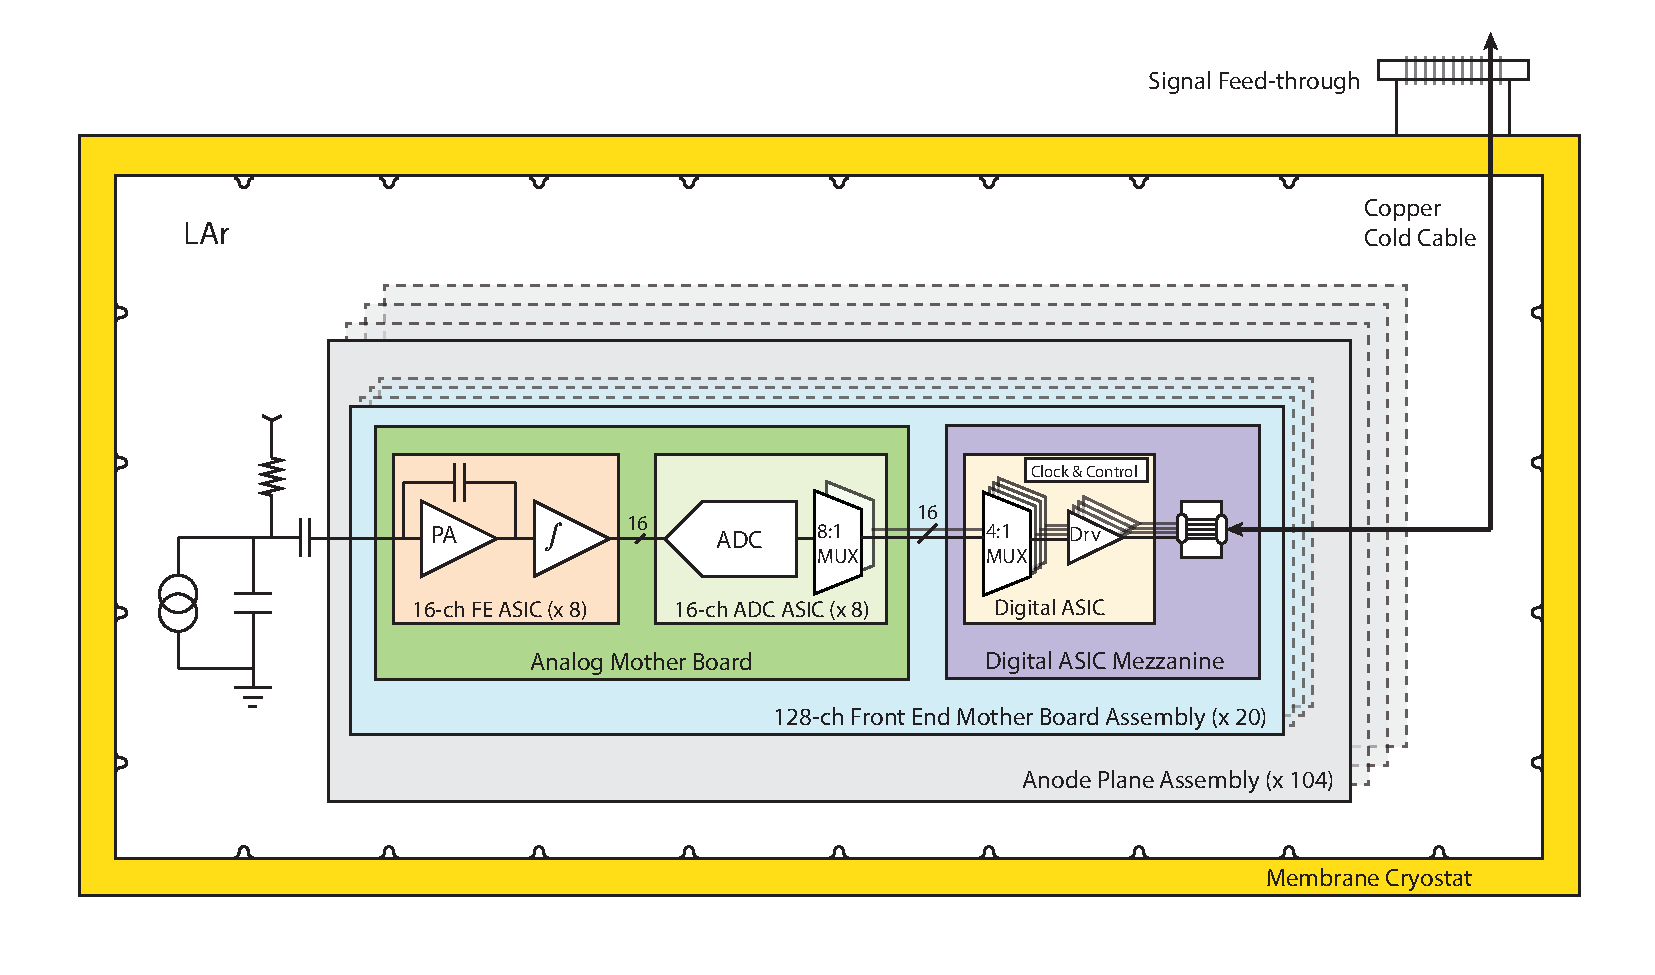
\includegraphics[width=\linewidth]{elect_schem.pdf}
\end{cdrfigure}

\begin{cdrfigure}[The Cold Mother Board (CMB), as used in the early set of tests]{elec_CMBpix}{The Cold Mother Board (CMB), as used in the early set of tests.
  {\bf Top:} The analog mother board, showing four ADC ASICs and four FE ASICs surface mounted.
  The other side of the board has another four ADC and FE ASICs.
  Except for anticipated small modifications, this board is essentially the final version.
  {\bf Middle:} The FPGA mezzanine, used in place of the digital ASIC mezzanine for the early set of tests.
  {\bf Bottom:} The complete CMB assembly as used in the early set of tests.
  The uppermost mezzanine board is the cable connection.}
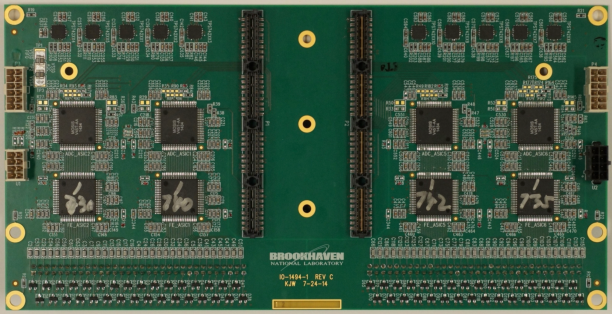
\includegraphics[width=0.65\linewidth]{elec_CMBpix1.pdf}
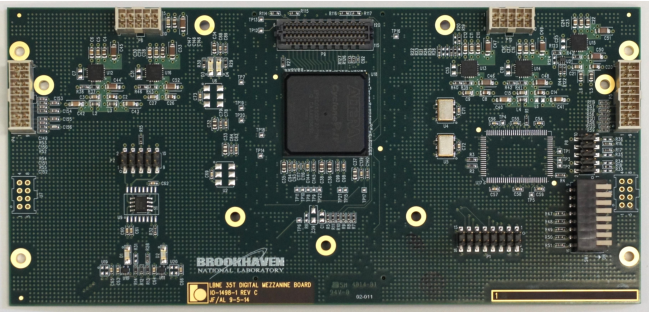
\includegraphics[width=0.65\linewidth]{elec_CMBpix2.pdf}
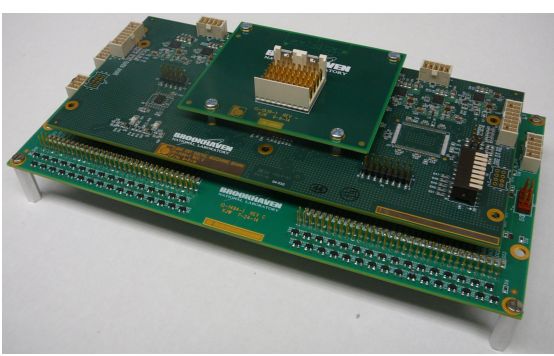
\includegraphics[width=0.65\linewidth]{elec_CMBpix3.pdf}
\end{cdrfigure}

The Cold Digital Data (COLDATA) ASIC and its voltage regulators are mounted on the digital ASIC mezzanine.
The COLDATA ASIC provides:
\begin{itemize}
\item The communication protocol with the data acquisition system (DAQ)
\item The control required to program and read out the FE and ADC ASICs
\item The system clock interface
\item Four 4:1 Muxs that combine 16 serial lines from the ADCs of eight channels each into four serial lines of 32 channels each
\item Four 1-Gbps serial drivers that form the data link to DAQ
\end{itemize}
If it is demonstrated that the COLDATA ASIC can achieve 2~Gbps,
then the 4:1 Mux will be increased to 8:1 and only two serial drivers will be implemented,
with a subsequent reduction in cabling, etc.
In either case, the data rates will not be high enough to require the use of optical fibers in the cold,
nor is there a need for zero suppression or data compression.
This greatly reduces the complexity of the COLDATA ASIC, with a corresponding decrease in overall risk,
including risk of failure-to-implement (within a fixed schedule and budget)
and risk of device failure during long-term operation.
Data will be driven to DAQ through copper cable utilizing low-voltage differential signaling (LVDS).
Output data cables will go to a signal feedthrough and from there to an external crate mounted nearby.
Under DAQ scope, further data processing is done in the external crate
and data is transmitted via optical fiber to front-end computers.

% 2015-02-27 chc: remove reference to the outdated block diagram
%Figure~\ref{fig:elec_asic_layout} shows a block diagram of the proposed 16-channel front-end ASIC.
The analog FE ASIC has 16 channels.
Each channel includes a charge amplifier with a gain selectable from one of 4.7, 7.8, 14 and 25~mV/fC
(full scale charge of 55, 100, 180 and 300~fC),
a high-order anti-aliasing filter with adjustable time
constant (peaking time 0.5, 1, 2, and 3 $\mathrm{\mu}$s),
an option to enable AC coupling,
and a baseline adjustment for operation with either the collecting or the non-collecting wires.
The 16-channel FE ASICs then transmit the shaped pulse to a 16-channel 12-bit 2~MS/s ADC ASIC.
Shared among the 16 channels in the FE ASIC are the bias circuits, programming registers,
a temperature monitor, an analog buffer for signal monitoring, and the digital interface.
The estimated power dissipation of FE ASIC is about 6~mW per channel at 1.8~V supply.
Shared among the 16 channels in the ADC ASIC are the bias circuits, programming registers,
an 8:1 Mux, and the digital interface
The estimated power dissipation of FE ASIC is below 5~mW per channel at 1.8~V supply.


%%%%%%%%%%%%%%%%
\section{CMOS Circuit Design}
\label{sec:fe_CMOS}

Compared to the situation at 300~K, charge-carrier mobility in silicon increases at 89~K
while thermal fluctuations decrease with $kT/e$.
These effects result in a higher gain (transconductance/current ratio = $g_{m}/ i$), higher speed, and lower noise
at 89~K than at 300~K.
For a given drain-current density, the same degree of impact ionization (measured by the transistor substrate current)
occurs at a somewhat lower drain-source voltage at 89~K than at 300~K.
The charge trapped in the gate oxide and its interface with the channel causes degradation in the transconductance (gain)
of the transistor and a threshold shift.
The former is of major consequence as it limits the effective lifetime of the device
(defined in industry and the literature as 10\% degradation in transconductance).
Thus, an MOS transistor has equal lifetime due to impact ionization at 89~K and at 300~K,
but at different drain-source voltages $V_{DS}$,
as illustrated in Figure~\ref{fig:LifetimetestVR}.  
This property can be exploited to stress the transistor with both increased current
and increased voltage while monitoring the substrate current and the change in $g_{m}$ due to impact ionization.
Under these conditions, the lifetime can be reduced arbitrarily by many orders of magnitude,
and the limiting operating conditions for a lifetime in excess of $\sim$20 years can be determined.
With this foundation, more conservative design rules (lower current densities and voltages)
can be derived and applied in the ASIC design.
With this accelerated testing the expected lifetimes can be verified for the several
widely available CMOS technologies under consideration (TSMC, IBM, AMS).
It should be noted that this is a standard test method used by the semiconductor industry;
it is used to qualify electronics for deep space NASA missions as well as commerical PCs.
 
\begin{cdrfigure}[Lifetime at different temperatures vs V$_{DS}$]{LifetimetestVR}{Lifetime at different temperatures vs V$_{DS}$}
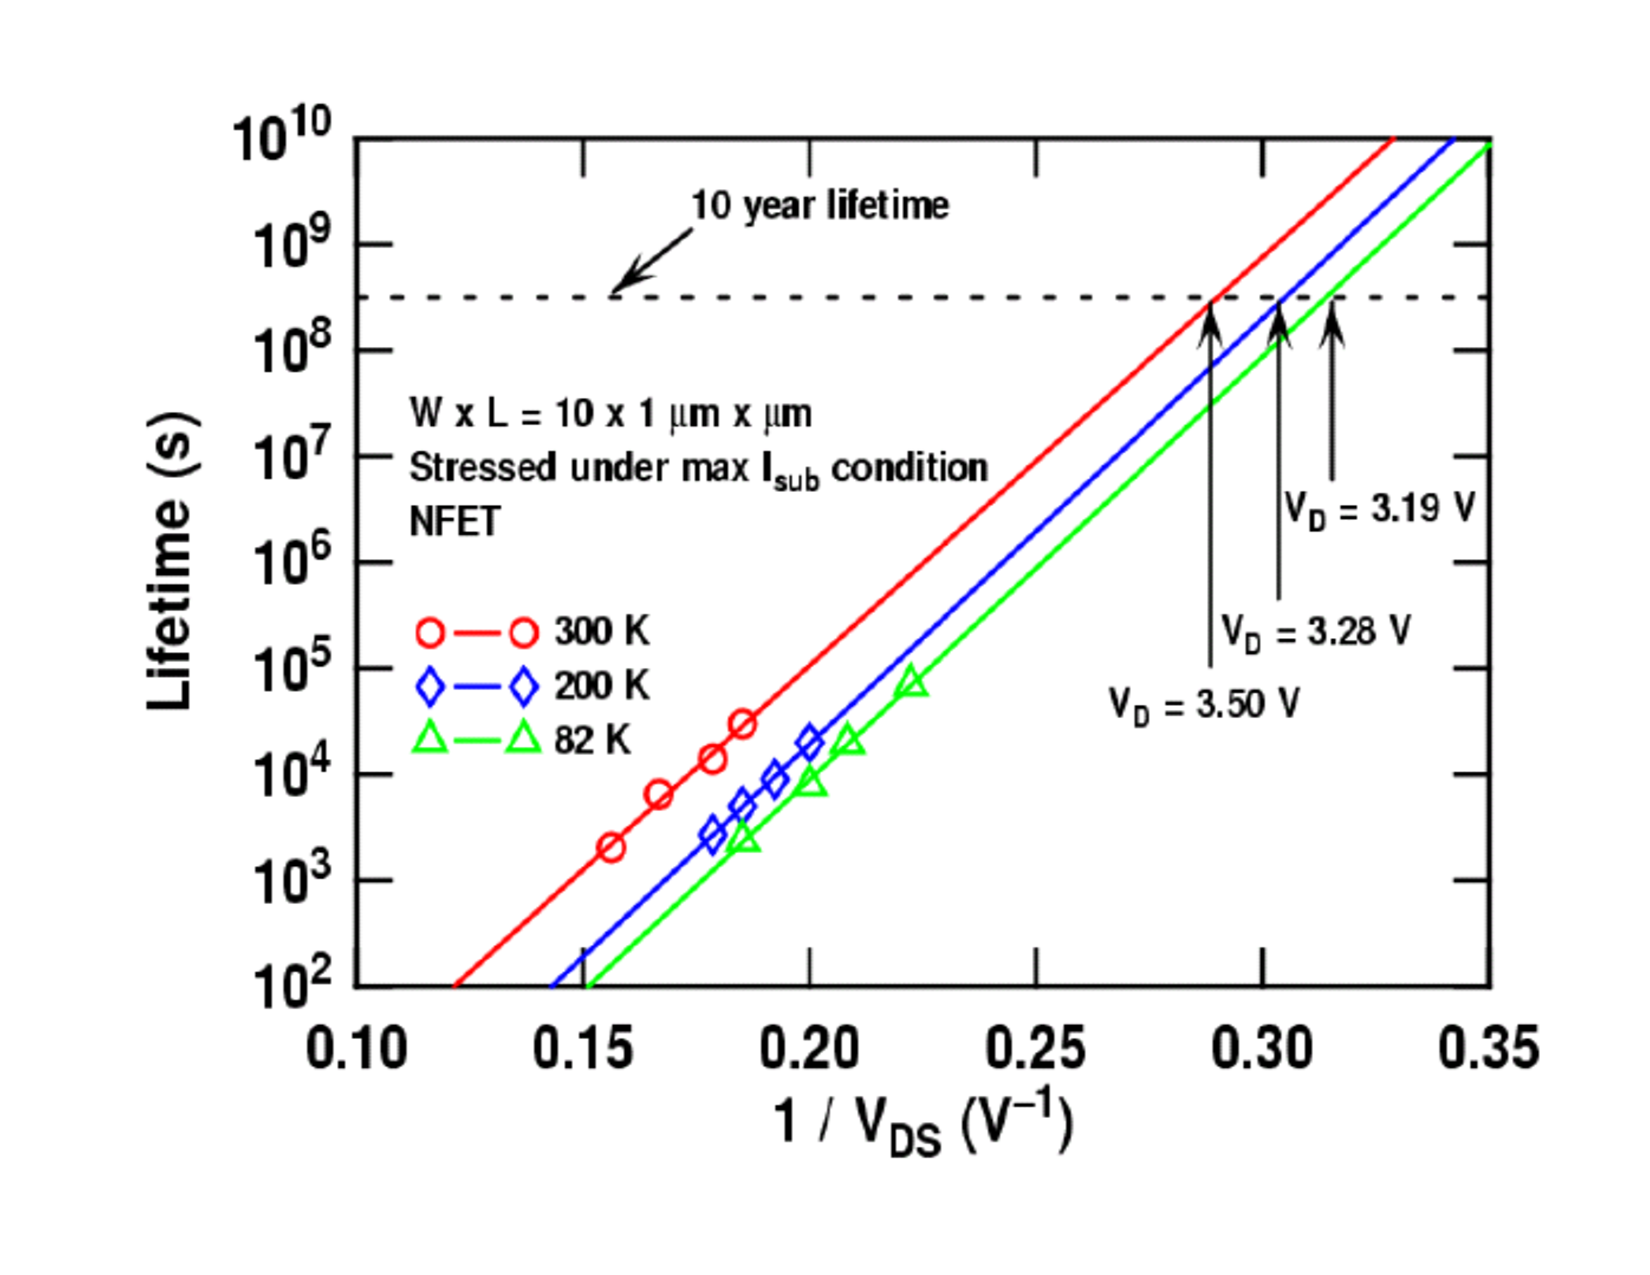
\includegraphics[width=0.9\textwidth]{LifetimetestVR}
\end{cdrfigure}

To successfully design CMOS circuits that will operate at cryogenic 
temperatures, two critical issues must be addressed and resolved. 
The first issue is the need for realistic models at the operating temperature 
of all active and passive components in order to reliably predict operating points,
signal response and noise during the design process.
The second issue is that the design must ensure a long operational lifetime, since once the TPC is filled 
with LAr the detector must operate for about 15~years without any access to the 
electronics for repair or replacement.
Concerning the availability of realistic models, 
our preliminary results from the cryogenic characterization (down to 40 K) of a complete 
mixed-signal ASIC \cite{CMOS-Compton} in a commercial CMOS 0.25~$\mu$m technology, 
originally developed for room-temperature applications, indicates that the models 
are useful to first order.
To refine these models, several 
single-transistor test structures were fabricated on the first prototype of the 0.18~$\mu$m device. 
Measurements of the properties of these structures at cryogenic temperatures 
have been used to refine the device models at 89~K. 

The lifetime of CMOS circuits is limited by several mechanisms which degrade 
the performance over time, eventually causing the circuit to fail to perform as specified. 
The rates of most degradation mechanisms in CMOS, such as electro-migration (EM), 
stress migration (SM), time-dependent dielectric breakdown (TDDB), thermal cycling (TC), 
and negative bias-temperature instability (NBTI), all scale with temperature such that 
cryogenic operation is favored \cite{CMOS-lifetime}\cite{PMOS-model}. The only mechanism 
that could affect the lifetime at cryogenic temperature is the degradation due to 
impact ionization, which causes charge trapping in the MOSFET gate oxide at 
large drain-current densities (the ``Hot Carrier'' effect). Results from a CMOS reliability study~\cite{CMOS-reliability} 
provide general design guidelines (for device geometry, bias and current density) 
that should guarantee a lifetime well in excess of 15~years for continuous cryogenic operation. 
These design guidelines also provide information for designing test conditions to observe the 
deterioration mechanism and to extrapolate from accelerated deterioration rates, 
measured under stressed conditions within practical times, to the ultimate lifetime under normal operation.

A monitor of the impact ionization is the bulk current, which reaches a maximum at $V_{DS} = V_{DD}$ and at $V_{GS} = 0.5 V_{DD}$.
When operating constantly in this condition at room temperature, a properly designed device 
will typically have a lifetime (defined as a 10\% degradation in $g_m$) of about 10~years. 
The bulk current (i.e., the impact ionization) increases by roughly a factor of four from 300~K to 77~K 
\cite{CMOS-reliability} and a circuit designed for operation at room temperature would have 
a proportionately shorter useful life at cryogenic temperature. As stated above, in order to guarantee 
the required lifetime at cryogenic temperatures, design guidelines must be modified for both analog 
and digital circuits. For analog circuits, this is done by operating the devices at moderate-to-low 
drain current densities, where impact ionization becomes negligible. 
%
For digital circuits, 
operating the devices with reduced $V_{DD}$ (about 20\%) and using non-minimum channel length L
is easily accommodated since at cryogenic temperature the speed of the digital circuit increases, 
compensating for the increased L.
%
These guidelines will be verified with accelerated aging tests, 
at increasing values of $V_{DD}$, on dedicated structures. Such tests also will be conducted on 
prototype samples throughout the development process to verify the long-term reliability of the final ASICs.

%
%%%%%%%%%%%%%%%%
\subsection{Cold Analog ASICs}
\label{subsec:fe_CMOS_analog}

The development of the readout ASIC has begun by designing and fabricating in a commercial CMOS
process (0.18~$\mu$m and 1.8V) a 16-channel ASIC implementing the complete analog front-end section.
The FE ASIC layout is shown in Figure~\ref{fig:elec_FE_ASIC}.
This process is expected to be available for at least another 10~years. 
The charge amplifier input MOSFET is a p-channel biased at 2~mA with a L/W (channel length/width) ratio
of 0.27~$\mu$m / 10~$\mu$m, followed by dual cascade stages.
The charge amplification and shaping filter have digitally programmable gain and peaking time
(as listed in Section~\ref{sec:fe_arch}).
Each channel also implements a high-performance output driver,
which is used to drive a long cable when it is used in a standalone mode, as it is in MicroBooNE.\cite{microboone-url}
The buffer can be disabled when it is interfaced to an ADC ASIC to reduce the power consumption.
The ASIC integrates a band-gap reference (BGR) to generate all the internal bias voltages and currents.
This guarantees a high stability of the operating point over a wide range of
temperatures, including cryogenic.
The ASIC is packaged in a commercial, fully encapsulated plastic QFP 80 package.

\begin{cdrfigure}[The layout of the 16-channel analog FE ASIC]{elec_FE_ASIC}{The layout of the 16-channel analog FE ASIC}
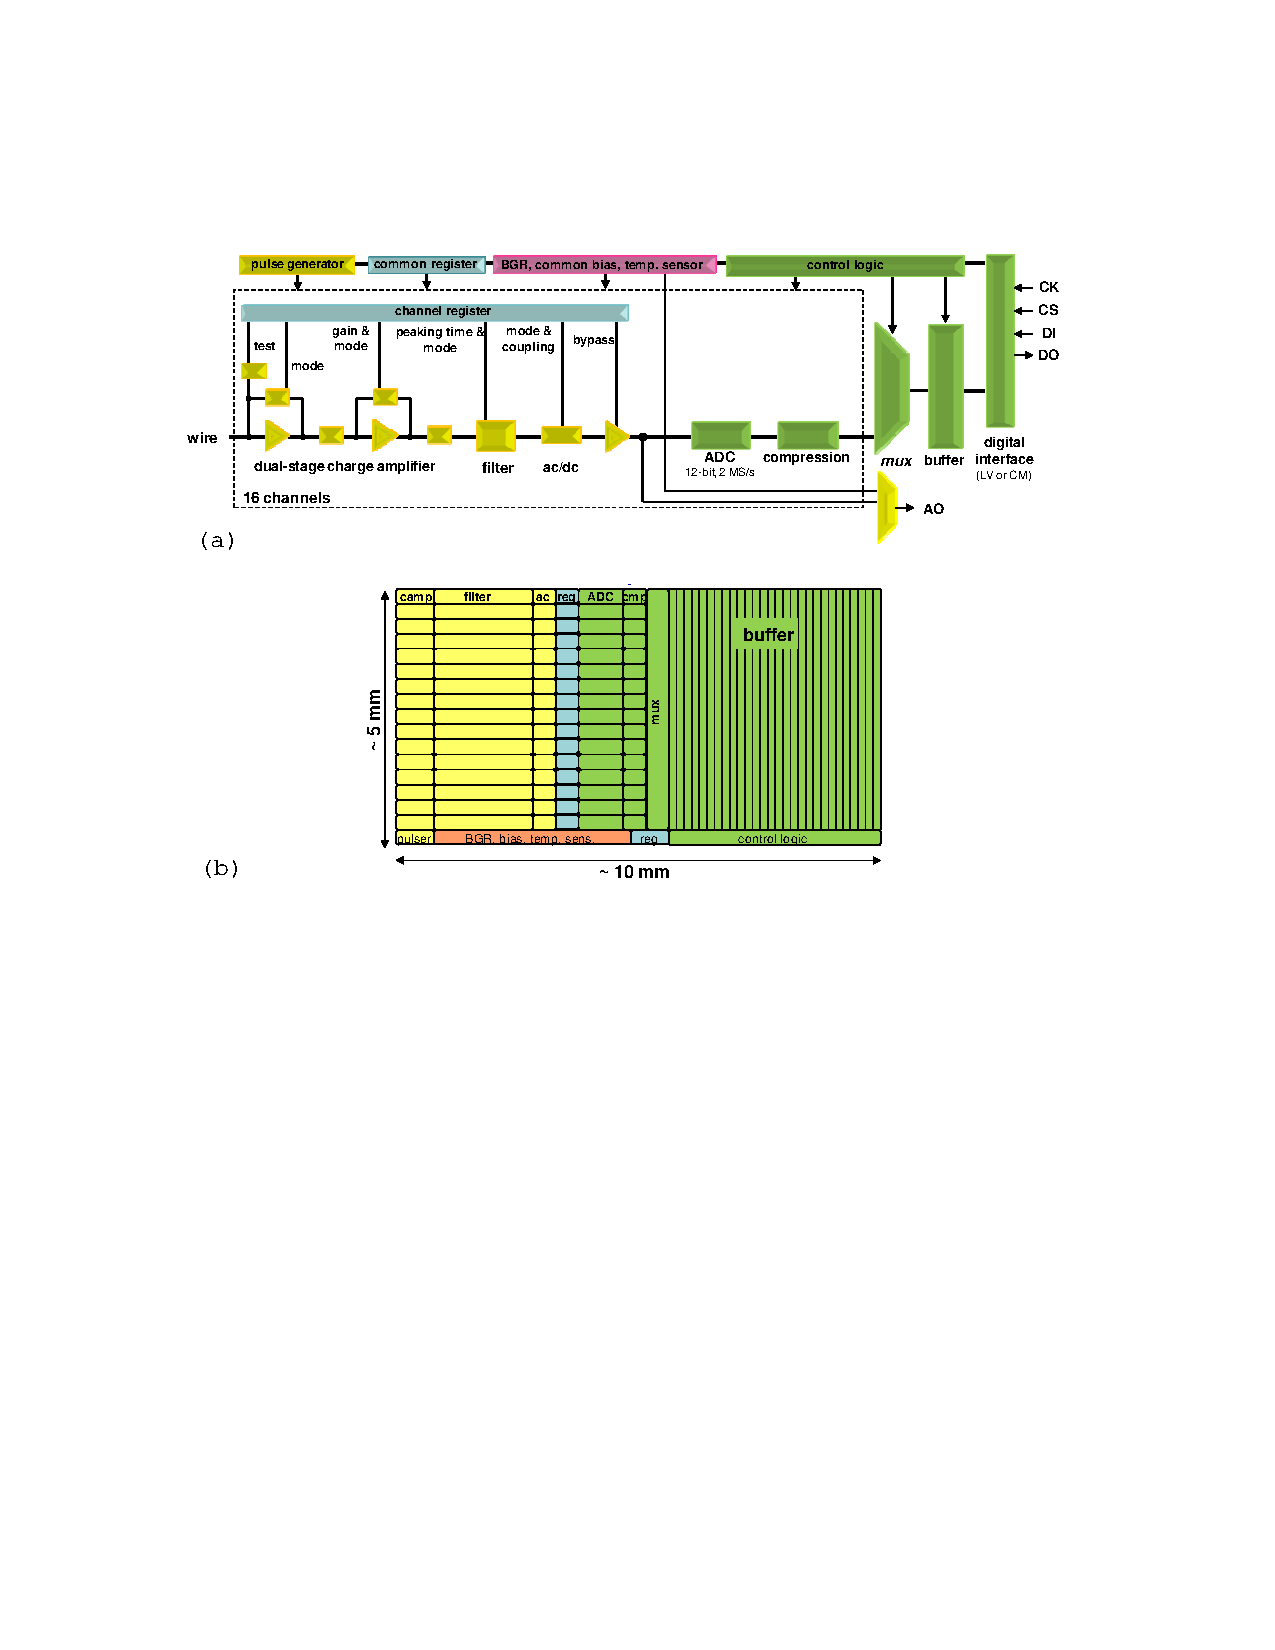
\includegraphics[width=\linewidth]{elec_FE_ASIC} % New one.
\end{cdrfigure}

This ASIC has now been through four design/fabrication/testing revision cycles.
Prototypes from each cycle have been evaluated and characterized at room (300~K) and liquid nitrogen (77~K) temperatures.
During these tests the circuits have been cycled multiple times
between the two temperatures and operated without any change in performance.
Figure~\ref{fig:ce_elec_shaper_out} shows the measured pulse response, along with
details on the adjustability of the gain, peaking time and baseline.
These results are in close agreement with the simulations and indicate
that both the analog and the digital circuits and interface operate as
expected in a cryogenic environment.
% 2015-02-27 chc: outdated information is removed
% Simulations and experimental results show that the pole-zero cancellation needs to be optimized,
% which will be done in the next revision of the design.
Also reported in Figure~\ref{fig:ce_elec_shaper_out} are the outputs of the BGR and temperature sensor,
which are in close agreement with the simulations as well.

\begin{cdrfigure}[Measured pulse response with details]{ce_elec_shaper_out}{Measured pulse response with details on gain, peaking time and baseline adjustments}
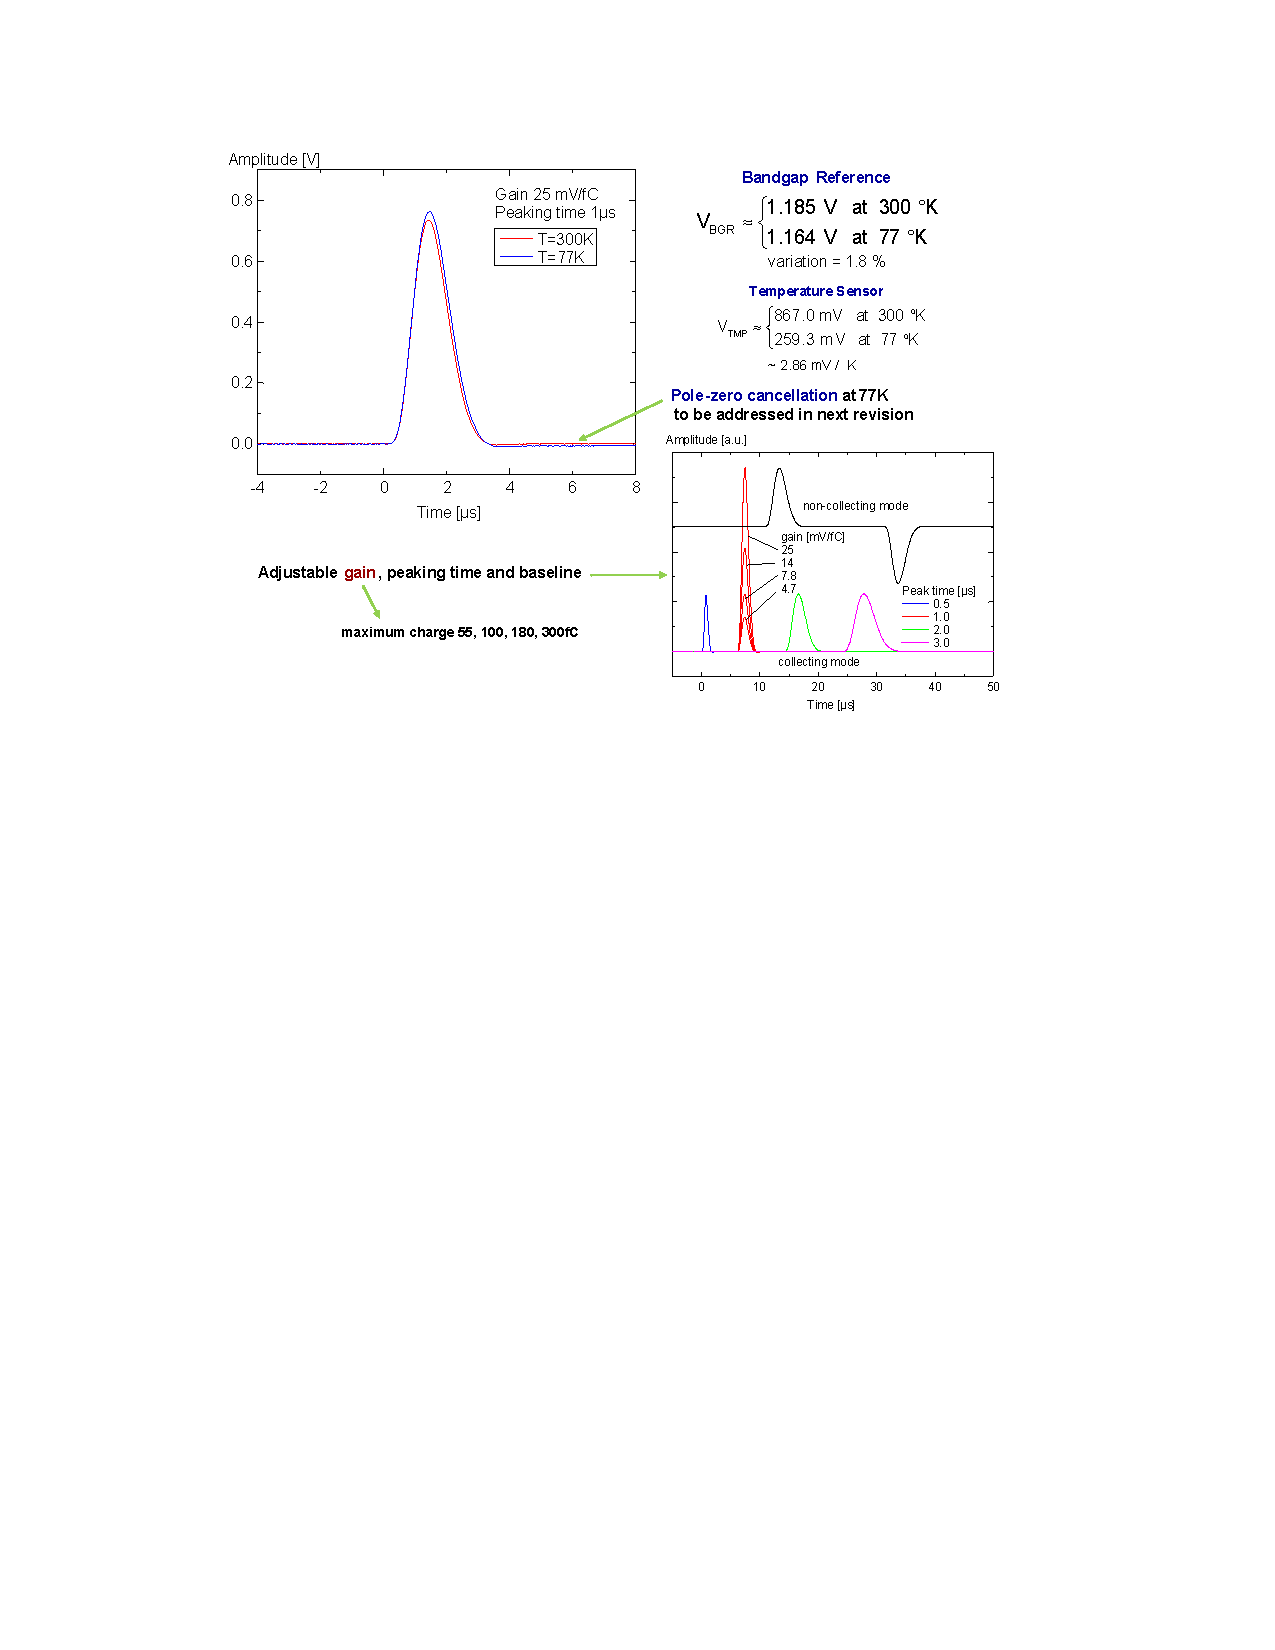
\includegraphics[width=\linewidth]{v5c3-cel-shaper-out.pdf}
\end{cdrfigure}

\begin{cdrfigure}[Measured ENC vs filter time constant]{ce_elec_enc}{Measured ENC vs filter time constant from the first two versions of the analog front end ASICs}
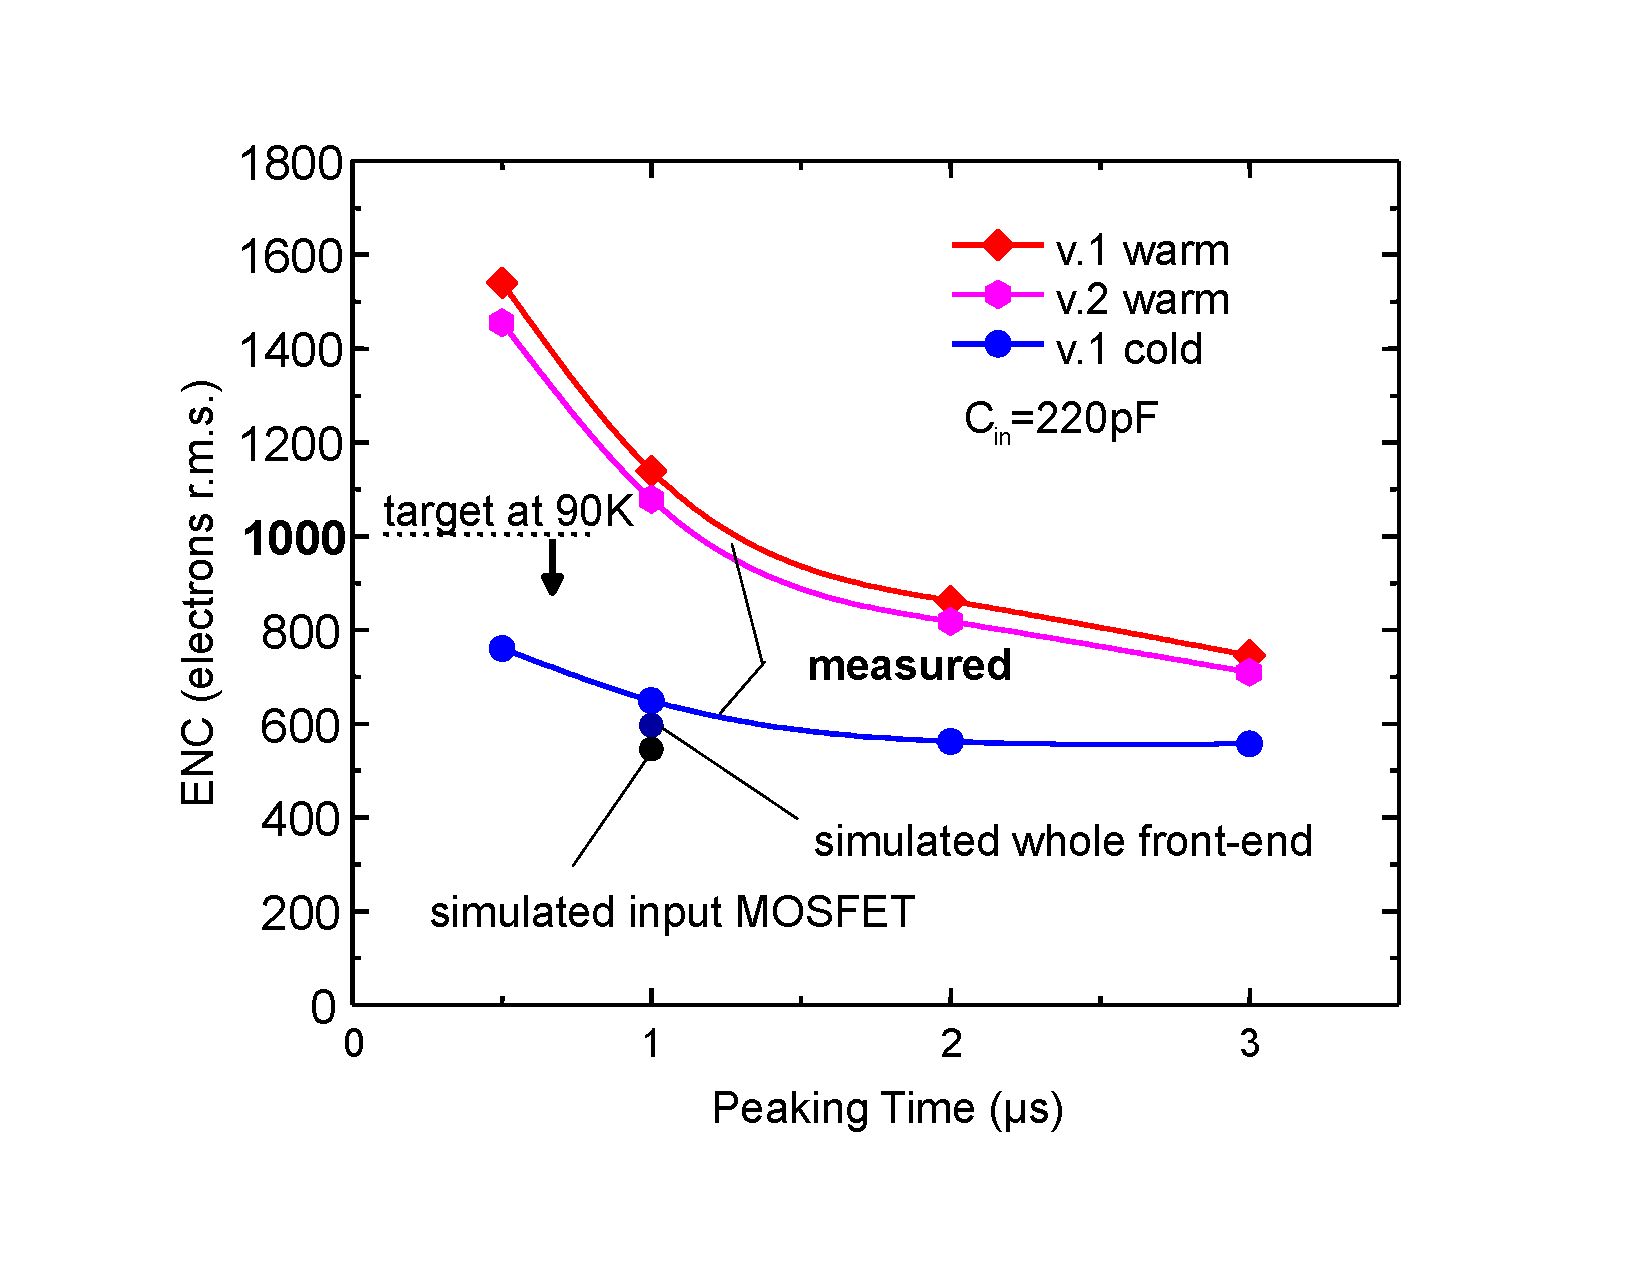
\includegraphics[width=4in]{v5c3-cel-enc.pdf}
\end{cdrfigure}

Figure~\ref{fig:ce_elec_enc} shows the measured ENC versus filter-time constant (peaking time).
At 1~$\mu$s about 650 e$^{-}$ was measured, to be compared to the simulated value of 500 e$^{-}$.
The difference is mainly due to the thermal noise from a $\sim$11-ohm parasitic resistance of the input
line (shown in the detail of Figure~\ref{fig:ce_elec_enc}), which contributes about 350 electrons at 77~K.
The width of the line has been increased in a revision in order to make this contribution negligible.
A second contribution, on the order of 100 e$^{-}$,
was due to the dielectric loss from the capacitor (220~pF) used to simulate the wire
(the cases of MICA and NPO ceramic were compared).
This contribution would not be present with the input connected to a sense wire in the TPC.

Each channel is equipped with an injection capacitor which can be used
for test and calibration and can be enabled or disabled through a
dedicated register. The injection capacitance has been measured using 
a calibrated external capacitor. The measurements show
that the calibration capacitance is extremely stable, changing from
184~fF at room temperature to 183~fF at 77~K. This result and the measured
stability of the peaking time demonstrate the high stability of the
passive components with the temperature. Channel-to-channel and chip-to-chip
variation in the calibration capacitor are typically less than 1\%. Measurements are being carried
out on the individual test structures fabricated on this ASIC to
confirm device models and design guidelines.

% 2015-02-27 chc: ADC ASIC is below
The development of the ADC ASIC is also using CMOS process (0.18~$\mu$m and 1.8V).
A 16-channel ASIC has been prototyped and tested.
The layout of the ADC ASIC is shown in Figure~\ref{fig:elec_ADC_ASIC}. 
The ADC ASIC has 12-bit resolution, 2~MS/s sampling rate, built in FIFO, two 8:1 multiplexing and two pairs of serialized output.
The ADC is a complex design, which has more than 300,000 transistors.
All of the transistor design has been done following the rules for long cryo-lifetime.

\begin{cdrfigure}[The layout of the 16-channel ADC ASIC]{elec_ADC_ASIC}{The layout of the 16-channel ADC ASIC}
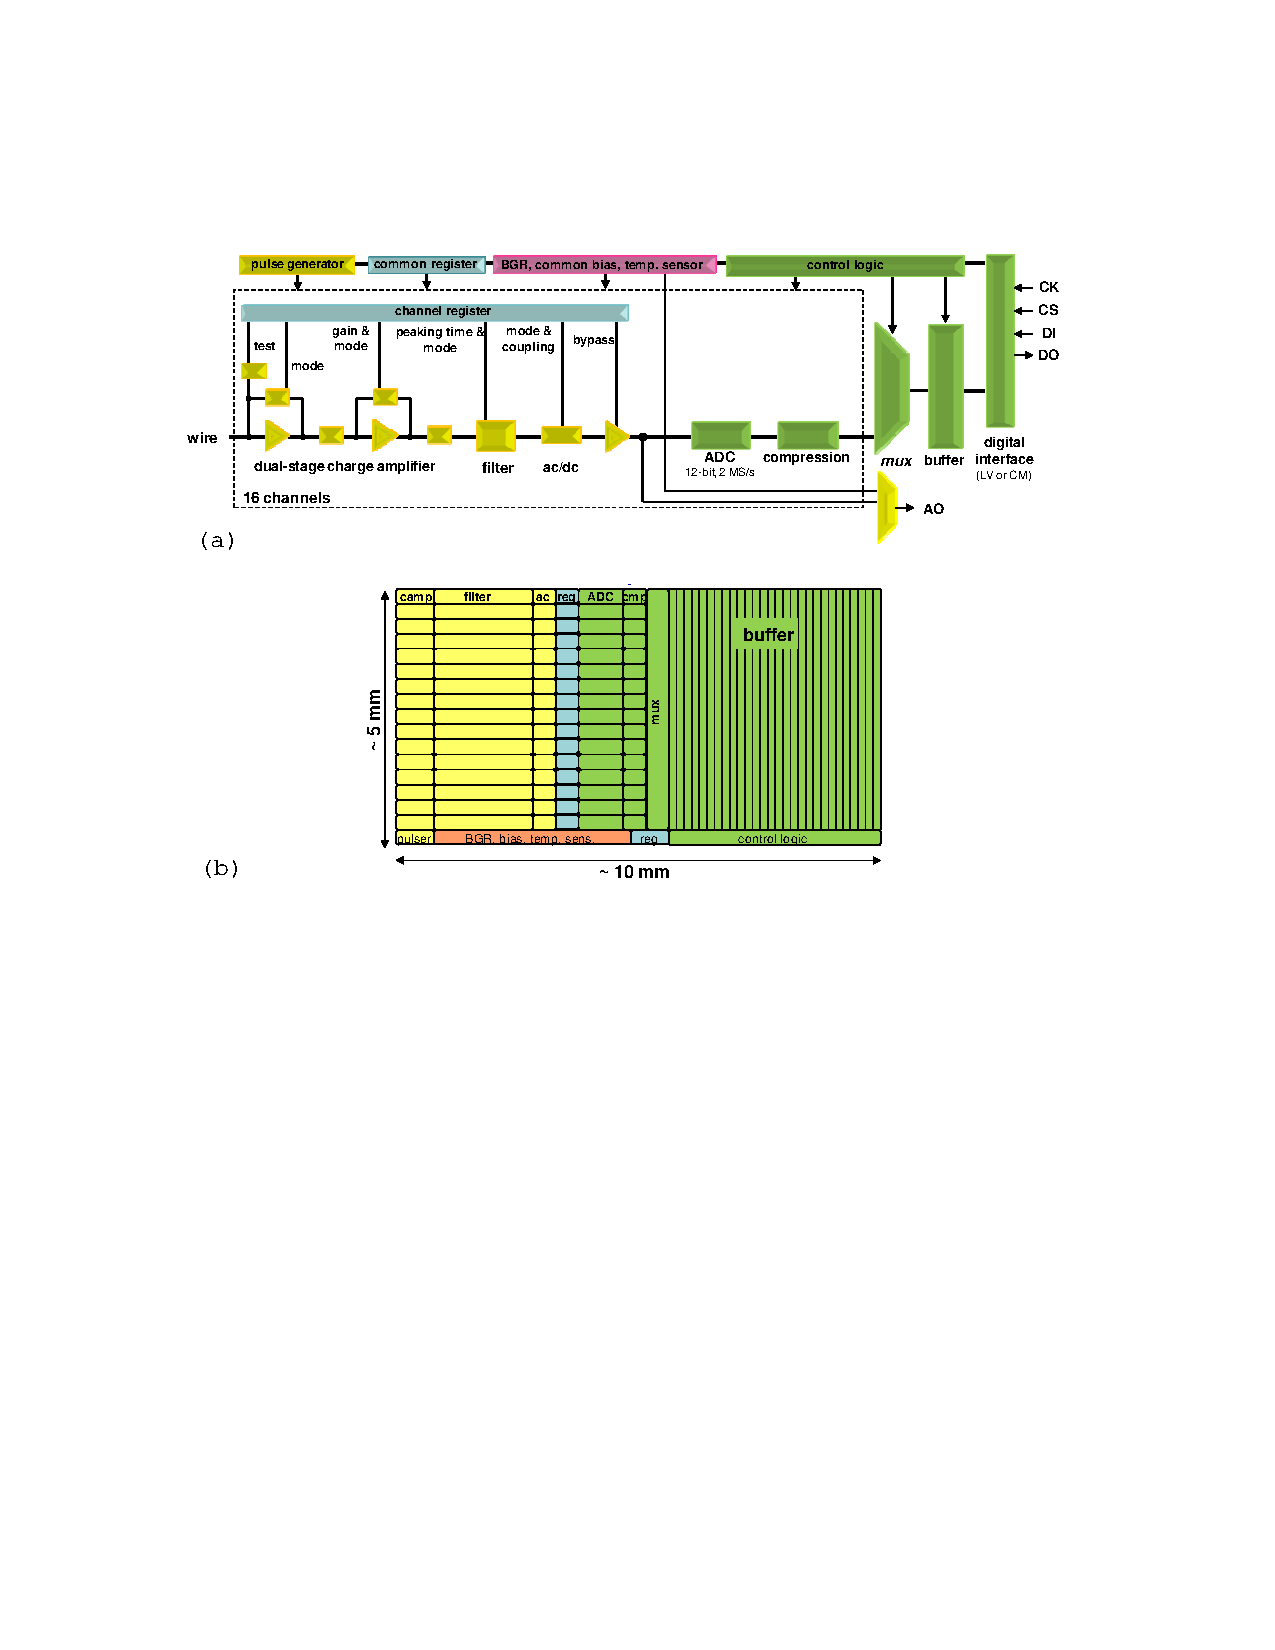
\includegraphics[width=\linewidth]{elec_ADC_ASIC} % New one
\end{cdrfigure}

The ADC ASIC has an input buffer with offset compensation to match the output of the FE ASIC.
The input buffer first samples the input signal (with a range of 0.2~V to 1.6~V),
then provides a current output after compensating for offset voltage error.
This current output is then supplied to the ADC which converts the input to digital in two phases.
The MSB (Most Significant Bit) 6~bits are first determined followed by the LSB (Least Significant Bit) 6~bits.
After the conversion the thermometer code is converted to binary and latched.
The output of ADC 16 can be monitored externally.
The data from the 16 ADCs is transferred in parallel to the FIFO block.
The built-in FIFO is 32~bits wide and 192~bits long,
it has the full and empty indicator flags to make it easy to interface to FPGA or digital ASIC.
The ADC along with the input buffers are biased internally using a bias generator and a bandgap voltage reference.
The bandgap voltage (VBGR) can be monitored and/or controlled externally.
It can be put in the low-power sleep mode, and woken up in less than 1~$\mu$s.

The ADC ASIC has now been through four design/fabrication/testing revision cycles.
Prototypes from each cycle have been evaluated and characterized at room (300~K) and liquid nitrogen (77~K) temperatures.
During these tests the circuits have been cycled multiple times.
The effective resolution with reference to the input referred noise is $\sim$11.6~bits at both 300~K and 77~K.
The differential non-linearity (DNL) is less than 4 LSBs for 99\% of ADC bins at both 300~K and 77~K.
The performance of the ADC meets the far detector requirements.

An analog front-end ASIC was adopted by the MicroBooNE experiment in 2010.\cite{microboone-url}
The fabrication and installation was successfully completed in early 2014, and now 
a total of 8,256 channels (516 FE ASICs) instrument the MicroBooNE TPC. 
A total of 2,048 channels (on 128 FE ASICs and 128 ADC ASICs) are used to instrument the 35-ton 
LArTPC.
The cold front-end mother boards have been produced and tested at 300~K and are currently
being tested at 77~K before final installation. % on the TPC.


%
%%%%%%%%%%%%%%%%
\subsection{Cold Digital Data ASICs}
\label{subsec:fe_CMOS_digital}

The development of the COLDATA ASIC will follow the same general guidelines developed for the cold analog ASICs, but
%The COLDATA ASIC design 
will differ from the analog design in a couple of aspects.
It is anticipated that the digital ASIC will make use of a 65-nm CMOS technology and require a
digital library with accurate cold timing models allowing for high-level language design and
automated place-and-route for design blocks using extensive digital logic.

\begin{cdrfigure}[Functional Block Diagram of the Cold Digital Data (COLDATA) ASIC]{elec_COLDATAfig}{Functional Block Diagram of the Cold Digital Data (COLDATA) ASIC}
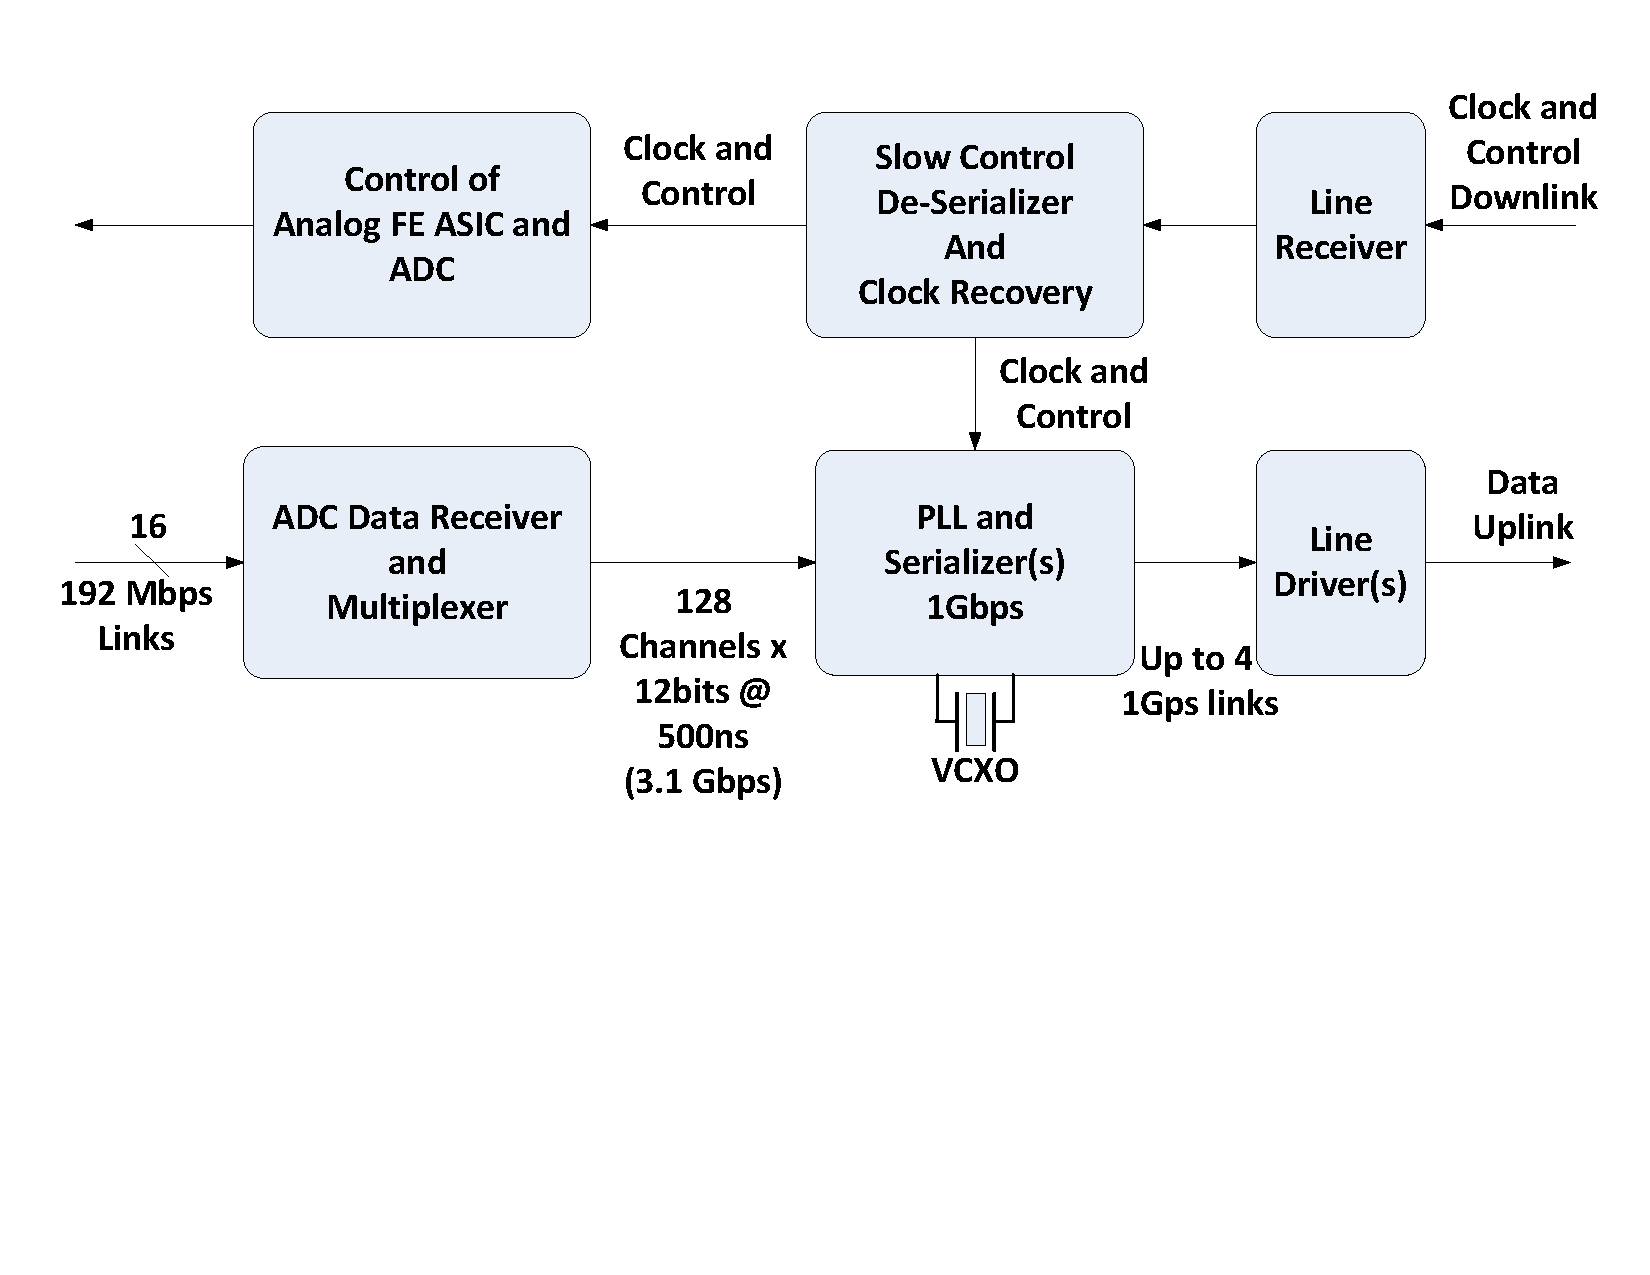
\includegraphics[width=6in]{elec_COLDATAfig.pdf}
\end{cdrfigure}

A block diagram of the COLDATA ASIC is presented in Figure~\ref{fig:elec_COLDATAfig}.
The major components of the COLDATA ASIC include a downlink which is required to receive the system clock and
the control/download information transmitted from the DAQ.
The download data must be transmitted to the FE and ADC ASICs on the CMB.
The system clock will provide a frequency reference to a crystal-based Phase Lock Loop (PLL)
which will generate a low-jitter stable clock to the high-speed serializer.

A single COLDATA ASIC on each CMB will also be receiving the data from each of the eight ADCs on a board.
Each ADC will transmit two streams of data at 192~Mbps for a total data input of 3.072~Gbps.
All data will be transmitted off-board to DAQ.
Twelve bits of ADC data per APA channel every 500~ns yields a single-channel bit rate of 0.024~Gbps.
With 8B10B encoding, for example, this increases to 0.03~Gbps, plus some overhead for frame data to indicate event blocks.
Assuming a conservative serial-link transmission speed of 1~Gbps, a single link can therefore handle 32 channels.
Thus, it is planned to drive four 1~Gbps links from each COLDATA ASIC.
A line driver will be designed that is capable of driving a copper link for the approximate 20~m required
to exit the LAr environment.
If a speed of 2~Gbps can be achieved, which is possible but not yet demonstrated,
the number of serial links for data transmission will be cut in half.

%
%%%%%%%%%%%%%%%%%%%%%%%%%%%%%%%%
\section{Signal Feedthroughs, Cabling, and Power}
\label{sec:ce_feedthrough}

A single type of feedthrough, henceforth ``signal feedthrough'', will handle the signals, supply voltages and control lines.
The TPC data rate per APA, using the full event-buffer scheme described earlier,
is sufficiently low that it is within the capability of a single LVDS channel on copper,
with an overall 32:1 Mux and 80 LVDS channels per APA.
There is, therefore, no need for high-speed optical links inside the cryostat, so all cables inside the cryostat will be copper.
This has the significant benefit of avoiding a major R\&D effort which would be required to demonstrate
both functionality and adequate lifetime of optical converters in LAr.
In addition to the high-speed data-output channels,
LVDS connections will be made to each APA to distribute a clock signal and control information.
These data can be transmitted at a lower bit rate.
Optical fiber will be employed externally to the cryostat, under DAQ scope.

%
%%%%%%%%%%%%%%%%
\subsection{Signal Feedthroughs }
\label{subsec:ce_feedthroughs}

No specific design for the Far Detector signal feedthroughs exists at this time.
We are currently exploring the possibility of working in tandem with the Near Detector group, which has
similar feedthrough needs. This group is starting with a concept based on the feedthrough design that has been successfully
running in the Atlas experiment for about 15 years\cite{ATLASFT}, demonstrating both longevity and reliability.
A somewhat different conceptual design of a signal feedthrough flange is shown in Figure~\ref{fig:ce_feedthrough}.
Based on a standard 8-in conflat flange with all commercial off-the-shelf components,
each of these feedthroughs would serve the bias/power/digital IO needs of two APAs.  

All cables inside the cryostat will be attached to their corresponding feedthroughs distributed throughout the cryostat roof.
The other ends of the cables will be connected to the matching connectors on the APAs in the cryostat.
The cables for the lower APAs must be carefully threaded through the hollow frames of the APA stacks;
these cables will be strain-relieved on the mounting rails above the APAs. 

% All data, control, bias and power supply lines will be duplicated to
% provide redundancy to avoid the loss on an entire APA.
% Two APAs will be cabled to one feedthrough in ``chimneys'' in the roof of the cryostat that
% contain the support rods for the TPC planes.

\begin{cdrfigure}[Conceptual design of signal/power feedthrough]{ce_feedthrough}{A conceptual design of a signal/power feedthrough using all off-the-shelf commercial components}
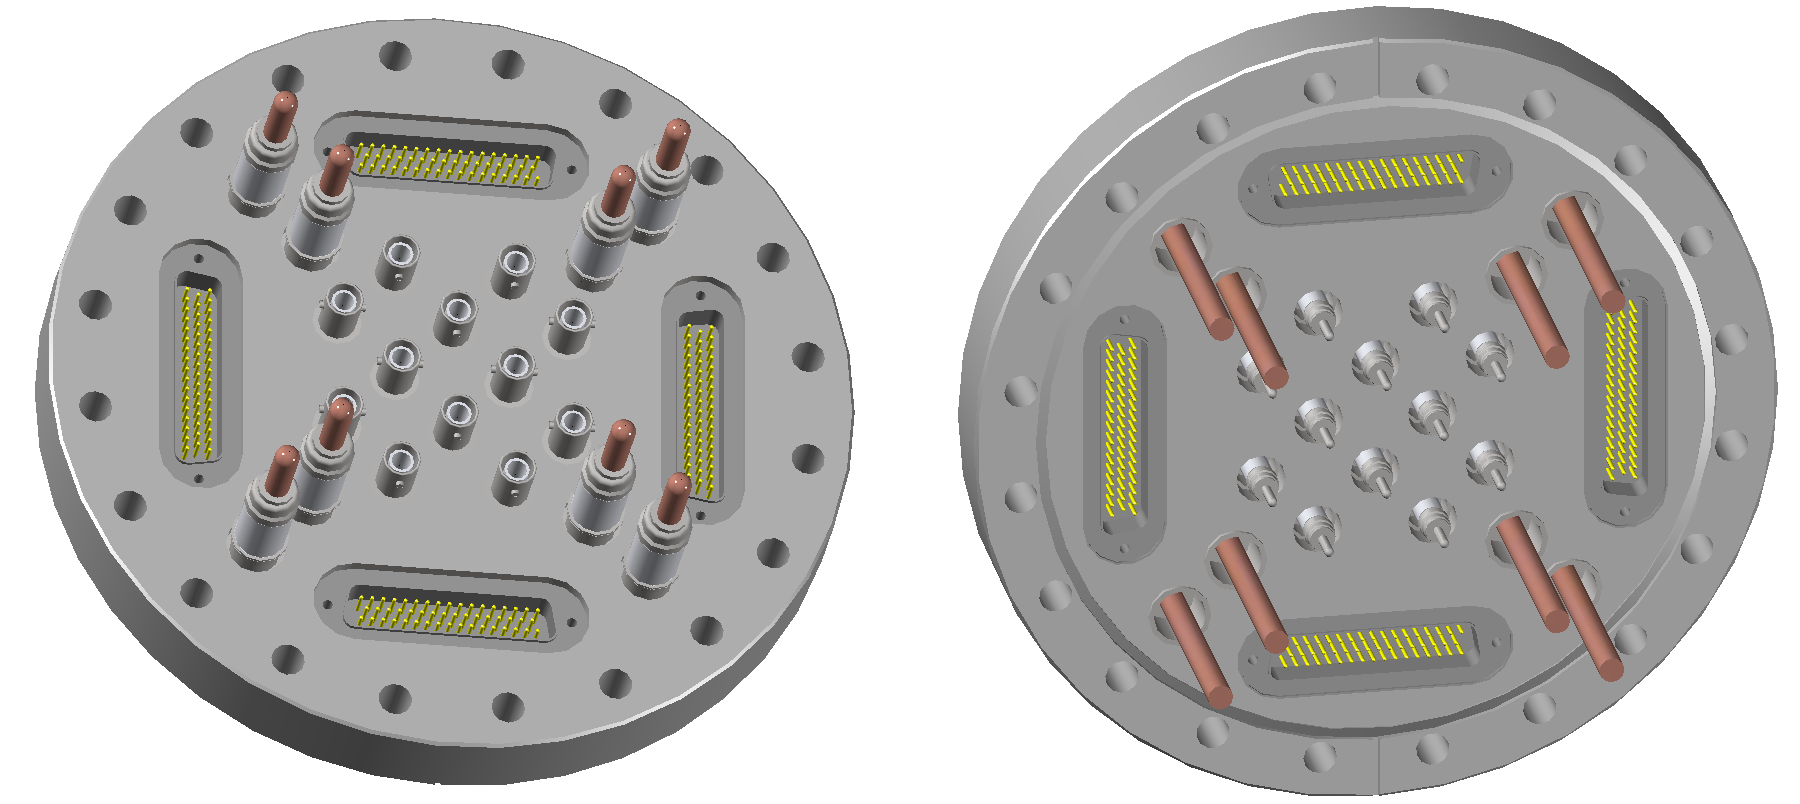
\includegraphics[width=\linewidth]{v5c3-signal-FT.png}
\end{cdrfigure}

The 35-ton prototype detector requires a feedthrough and cable plant similar to what a single full-size APA
will require and can serve as a model for at least one possible solution to the feedthrough problem.
In the 35-ton case, a custom printed circuit embedded in a single 10-in Conflat flange handles all the cabling
associated with the TPC and photon detector cabling as well as a small number of cables for a specialized
camera system to monitor the cathode connection.
For the 35-ton APAs there are, in addition to the TPC bias voltages, 16 cold electronics boards with data,
power and control wires plus some 74 photon detector signals on individual cables.
For a full-size far detector APA there would be 20 electronics boards with simpler control and power wiring
requirements and rather fewer photon detector cables so the 35-ton feedthrough will serve as a good model
for what might be done for the far detector.
While the electrical connection requirements are straightforward,
the reliable gas tightness of the flange with an embedded circuit board needs to be fully verified.
Also the planned method of reducing contamination from the cable plant in the ullage
(the warmer gas phase at the top of the cryostat) 
needs to be studied carefully, as does that for the 35-ton cryostat,
which has a has a much larger ullage than that planned for the far detector.


\begin{cdrfigure}[The 35 Ton ``Flange Board'', without the Conflat flange]{ce_feedthrough}{Photograph of the 35 Ton ``Flange Board'', without the Conflat flange which will be epoxy potted near
  the center of the printed circuit.
  This board carries all the electrical connections for the four small APAs in the 35 Ton
  test cryostat and is similar to the number of connections needed for a Far Detector APA}
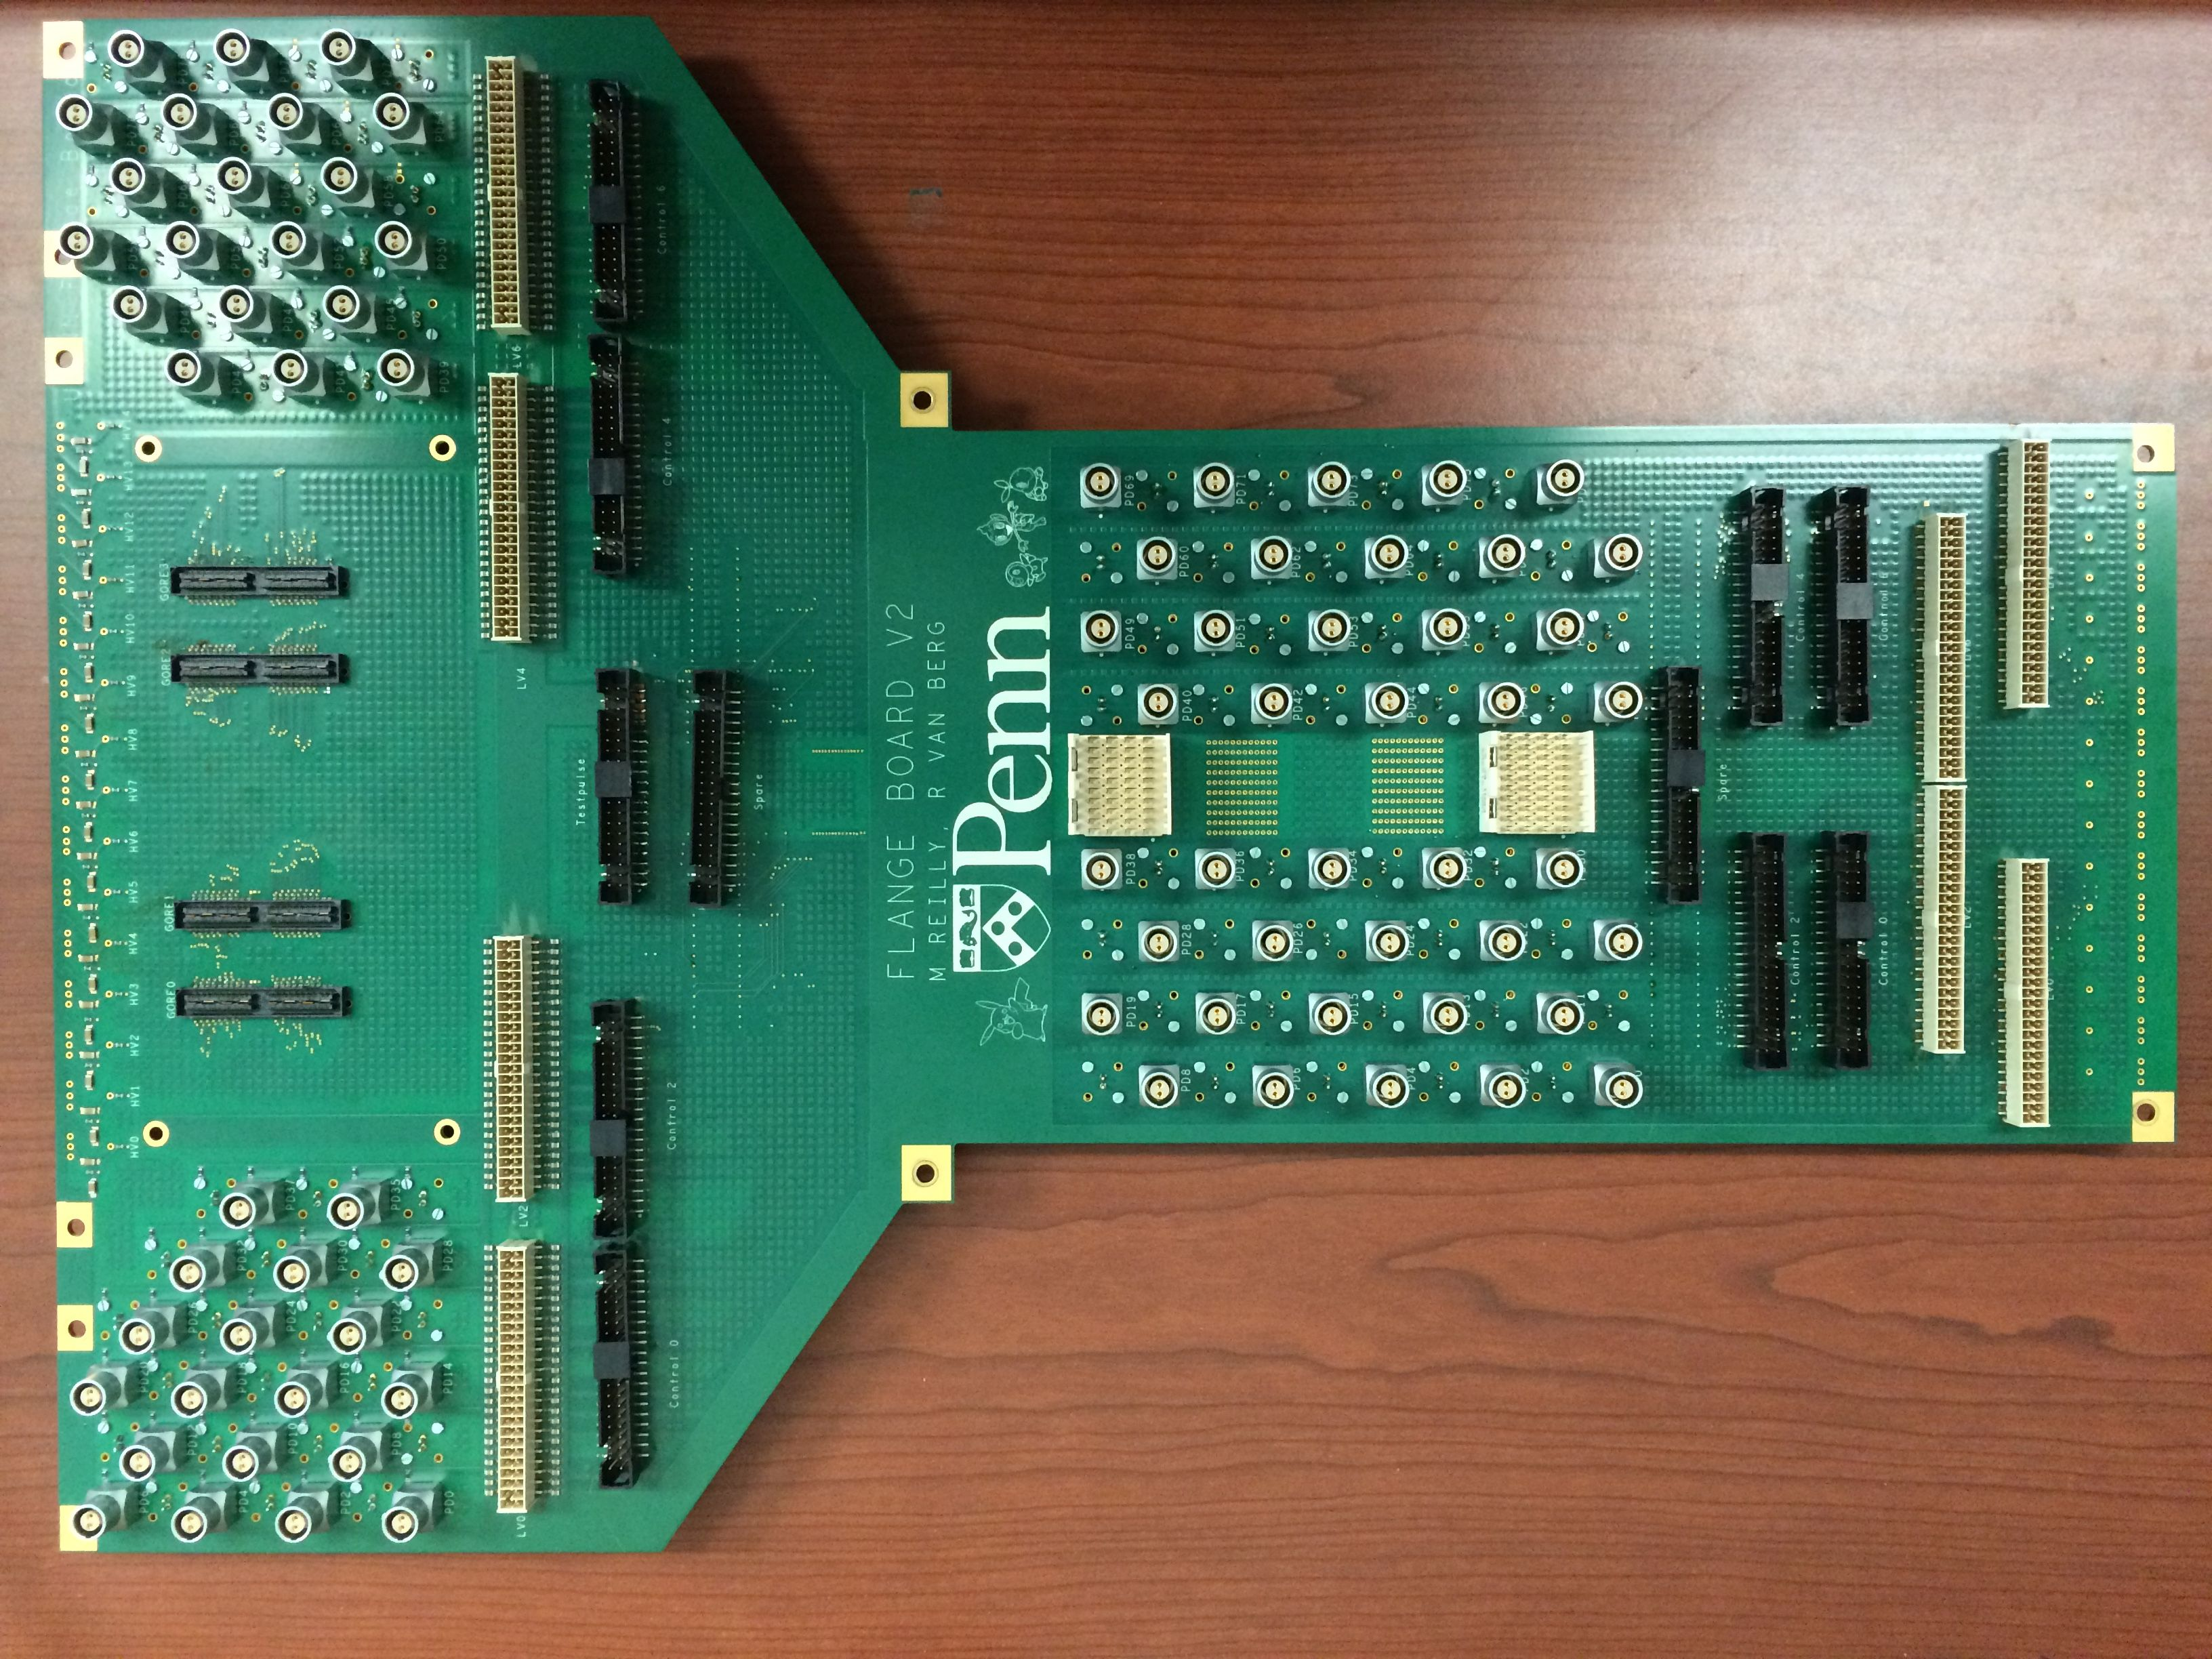
\includegraphics[width=\linewidth]{FlangeBoard.jpg}
\end{cdrfigure}

Measurements in the Materials Test Stand at Fermilab (described in Section~\ref{sec:mts})
have shown that impurities (principally O$_2$ and H$_2$O) embedded in objects submerged in the liquid argon do not result
in a decrease in electron-drift lifetime, whereas impurities in objects located in the ullage do.
This indicates the importance of minimizing the amount of material in the ullage.
It also indicates that it would be desirable to connect all cables to feedthroughs below the liquid surface,
and then pass the cables out of the cryostat, through an evacuated volume that traverses the gas and cryostat insulation,
to a matching set of feedthroughs to the outside.
In the 35-ton design, a stainless steel tube surrounds the cable bundle in the ullage and is partially sealed off below the
liquid level to limit contamination.
Understanding whether a scheme like this would be sufficient for the longer drift lengths in the far detector
is an important question to be addressed.

%
%%%%%%%%%%%%%%%%  
\subsection{Cabling for the Cold Electronics }
\label{subsec:ce_feedthrough_cable}

Five basic types of cables will be required to penetrate the cryostat and service the Cold Electronics.
We will require low-voltage cables to power the FE boards,
wire bias cables to provide the reference voltages for the wire planes,
moderate-speed cables for a communication downlink to the FE boards,
high-speed cables to carry the data out of the cryostat and signal cables to carry the photon detection out.
All of these cables will pass through the feedthrough port provided for each pair of stacked APAs.

The cables --- and connectors --- will be selected to have a low outgas and provide minimal contamination to the LAr environment.
%The same is true of connectors.
Connectors will also need to be tested for usage in LAr to make sure that a low ohmic contact is maintained
in the cryogenic environment.

We are looking into several types of cables and connectors.
The low-voltage cabling will be %defined by 
chosen based on power needs and whether we decide to go with a higher-voltage/lower-current
feed using DC/DC convertors or a low-voltage/higher-current feed used by low-voltage regulators.
Studies will take place to decide the most efficient and practical usage.

The wire-bias cables must deliver voltages up to %a couple  
two or three thousand volts with less than a couple of milliamps.
We anticipate using a coaxial cable and connectors which have been tested and found sufficient to provide this load.

The cables for the moderate speed downlink could utilize LVDS signaling and low-skew pairs.
Again, testing will be required to %identify and 
select the final cable and connectors.

For the high-speed data links, we anticipate using a low-skew copper twinax cable.
We have prototyped such a cable and found that we can drive data at 2~Gbps for a 20~m length.

Finally, the photon detector cables currently make use of shielded twisted pair cables which carry both
the DC bias voltage as well as the signals.
Future work involving these cables is described in Chapter~\cite{ch:photon}.

It will be important that all cables and connectors be somewhat rugged,
locking and able to withstand a minimum of several tens of mating cycles.
This is in addition to concerns about material compatibility and the fact they must work in the cryogenic environment.

%
%%%%%%%%%%%%%%%%
\subsection{Power for the Cold Electronics }
\label{subsec:ce_feedthrough_power}

The power-per-channel for the FE ASIC is designed to be about 15~mW and the total high-voltage
power requirement for each APA is expected to be about 65~W. 
Power will be supplied to the electronics on each APA separately by low-noise
power supplies outside the cryostat, either directly by
low-voltage (1.8~V), high-current (36 A) conductors or by high-voltage (48~V)
low-current (2~A) conductors to DC-DC converters placed locally in the LAr.
The use of DC-DC converters requires conductors with smaller cross section,
minimizing heat input to the cryostat (and ice formation on the feedthroughs).
However, the power dissipated by the (somewhat inefficient) converters in
the LAr will create boiling which may introduce contamination directly into the 
high-purity LAr, and if enough LAr is vaporized, may also produce strong mixing of the
ullage gas, driving more impurities into the liquid.
These effects of boiling LAr, unless they can be demonstrated to be harmless,
will drive a preference for eliminating DC-DC converters, and directly powering the front-end readout boards.

Heat conduction through the high-current feedthroughs and the self-heating ($I\cdot R$) of the wires are the factors
contributing to additional heat load on the cryogenic system.
The sum of the these two factors as a function of the wire gauge, however, has a minimum 
due to the two opposing dependencies on the copper-wire cross section.
An optimum wire gauge can be chosen to minimize heat input to the cryostat.
%
%%%%%%%%%%%%%%%%
\subsection{Wire-Bias Voltages}
\label{subsec:ce_feedthrough_wirebias}

Each anode plane assembly requires three bias voltage connections 
at $+$820V, $-$370V, and $-$665V.
The current on each of these supplies is expected to be zero at normal operation.
However the ripple voltage on the supply must be carefully controlled 
to avoid noise injection into the front-end electronics.  

The power supplies for the wire bias will be similar to 
those used for conventional multi-wire proportional chambers. 
Additional filtering networks will 
be needed to further reduce voltage ripples.  
The default feedthroughs are the commercial SHV type.  
However,  other, higher-density multi-channel 
feedthroughs capable of withstanding the maximum voltage are under investigation.  

%
%%%%%%%%%%%%%%%%%%%%%%%%%%%%%%%%
\section{CE Installation}
\label{sec:ce_install}

Cold electronics will be mounted on the TPC and installed inside the cryostat.
Because access to the cold electronics is not possible after the cryostat is sealed,
a full complement of tests will be performed during the development stage and before the final installation
(Figure~\ref{fig:elec_CMBonAPA}).

%%%%%%%%%%%%%%%%
\subsection{Prototype Testing}
\label{sec:ce_install_proto}

Dedicated test boards for the FE ASIC and ADC ASIC,
were used to characterize the performance of prototype ASICs at both 300~K and 77~K,
and taking them through multiple thermal cycles.
An automated test board was built for the FE ASIC to evaluate large numbers of FE ASICs at room temperature,
and another such board is currently being designed for the ADC ASIC.

The development of the FE and ADC ASICs has proceeded through a series of prototype designs.
A 128-channel prototype analog mother board has been developed and tested in the lab.
Together with an FPGA mezzanine in place of the digital ASIC mezzanine,
they form a front-end cold mother board assembly for use in the 35-ton prototype TPC.
A test stand has been developed to test the front-end mother board assembly
using a commercial FPGA evaluation board as a mini-DAQ system.
All evaluation test data are stored on a desktop PC and analyzed to
determine whether the board is ready to be installed on the detector.

During the prototype testing, a procedure has been developed for the production test of the cold electronics boards.
This includes key parameters (gain, noise, non-linearity, etc.) that should be tested,
detailed steps of the test to collect data and extract these parameters,
and also the work flows to perform the test at both 300~K and 77~K.

Prototype cold electronics has been tested with prototype TPC and DAQ system,
to evaluate the performance of the APA assembly, and help the development of the DAQ software.
A vertical slice test has been used as the test bed for the integration test.
It is an important step to identify potential issues, check out system integration and performance
before the installation into the cryostat.

%%%%%%%%%%%%%%%%
\subsection{Assembly Testing}
\label{sec:ce_install_assembly}

The front-end readout boards will be thoroughly tested. A testing program has been identified:
\begin{itemize}
\item A small number of the ASICs will undergo a complete suite 
of tests, including thermal cycling to determine the batch yield.
\item If the yield is high ($>$ 95\%), all ASICs will be mounted 
on the front-end boards.
Tests will be performed on each board and bad chips replaced as needed.
\item If the yield is not high, an automated test fixture will be 
fabricated to validate every ASIC chip before mounting on the readout boards.
Board-level tests after mounting the ASICs will be conducted.
\item The fully assembled front-end boards will be thermally cycled multiple times while connected
to a simple DAQ system to ensure reliable operation.
\item After the front-end electronics boards have been installed on an APA,
an initial calibration of all electronic channels will be performed.
The electronic gains and noise levels of all channels will be recorded in a database.
\item Electronic calibration on all channels will be performed while the APA is cold and again after it is warmed up.
Significant differences in the cold and warm calibration results will be investigated and remediated.  
\end{itemize}

%
%%%%%%%%%%%%%%%%
\subsection{Commissioning } 
\label{sec:ce_install_commission}

During installation, the DAQ system will be running continuously.
As soon as each stack of APAs is connected to the pre-routed cables, 
a suite of calibration runs will be performed to validate that all connections have been made properly.
Repair or replacement at this stage will still be straightforward.

Following the installation of the APAs and the sealing of the cryostat,
another complete test will be performed to verify the integrity of the cold electronics before the filling with argon.
After the cryostat is filled with LAr and the detector is cooled down,
an electronics calibration test will be performed to evaluate
the detector performance prior to data taking.

%

